% ----------------------------------------------------
% -------- BAYSIS - Selected as Jam Effector ---------
% ----------------------------------------------------
\subsection{BAYSIS - Selected as Jam Effector}

List of strong corrs (.14 for $\eta$ and 0.5 for $r$ ...):

\noindent
\begin{table}[h!]
	\centering
	\begin{tabular}{c|l}  
		Category & Strong \\
		\\[-1em]
		\hline
		\\[-1em]
		Strasse & TMax, TAvg, SMax, SAvg, Cov, TLHGV \\ 
 		Kat & TMax, TAvg, SAvg \\ 
 		%Typ & \\
 		%Betei & \\
 		UArt1 & SAvg \\
 		UArt2 & SMax \\
 		%AUrs1 & \\
 		%AUrs2 & \\
 		AufHi & TMax, TAvg \\
 		%Alkoh & \\
 		%Char1 & \\
 		%Char2 & \\
 		%Bes1 & \\
 		%Lich1 & \\
 		%Lich2 & \\
 		%Zust1 & \\
 		%Zust2 & \\
 		%Fstf & \\
 		WoTag & TAvg, SMax, Cov, TLHGV \\
 		%FeiTag & \\
 		Month & TMax, TAvg, SMax, SAvg, Cov, TLHGV \\
	\end{tabular}
    \caption{List of incident variables and their strong correlated congestion variable from the congestion-accident matched data which are classified as \textit{Jam Effector}}
	\label{tbl:correlation_list_baysis_effector}
\end{table}

% \newgeometry{left=1.5cm,right=1cm}
% 	\pagestyle{empty}
% 	\begin{figure}[ht]
% 		\centering
% 		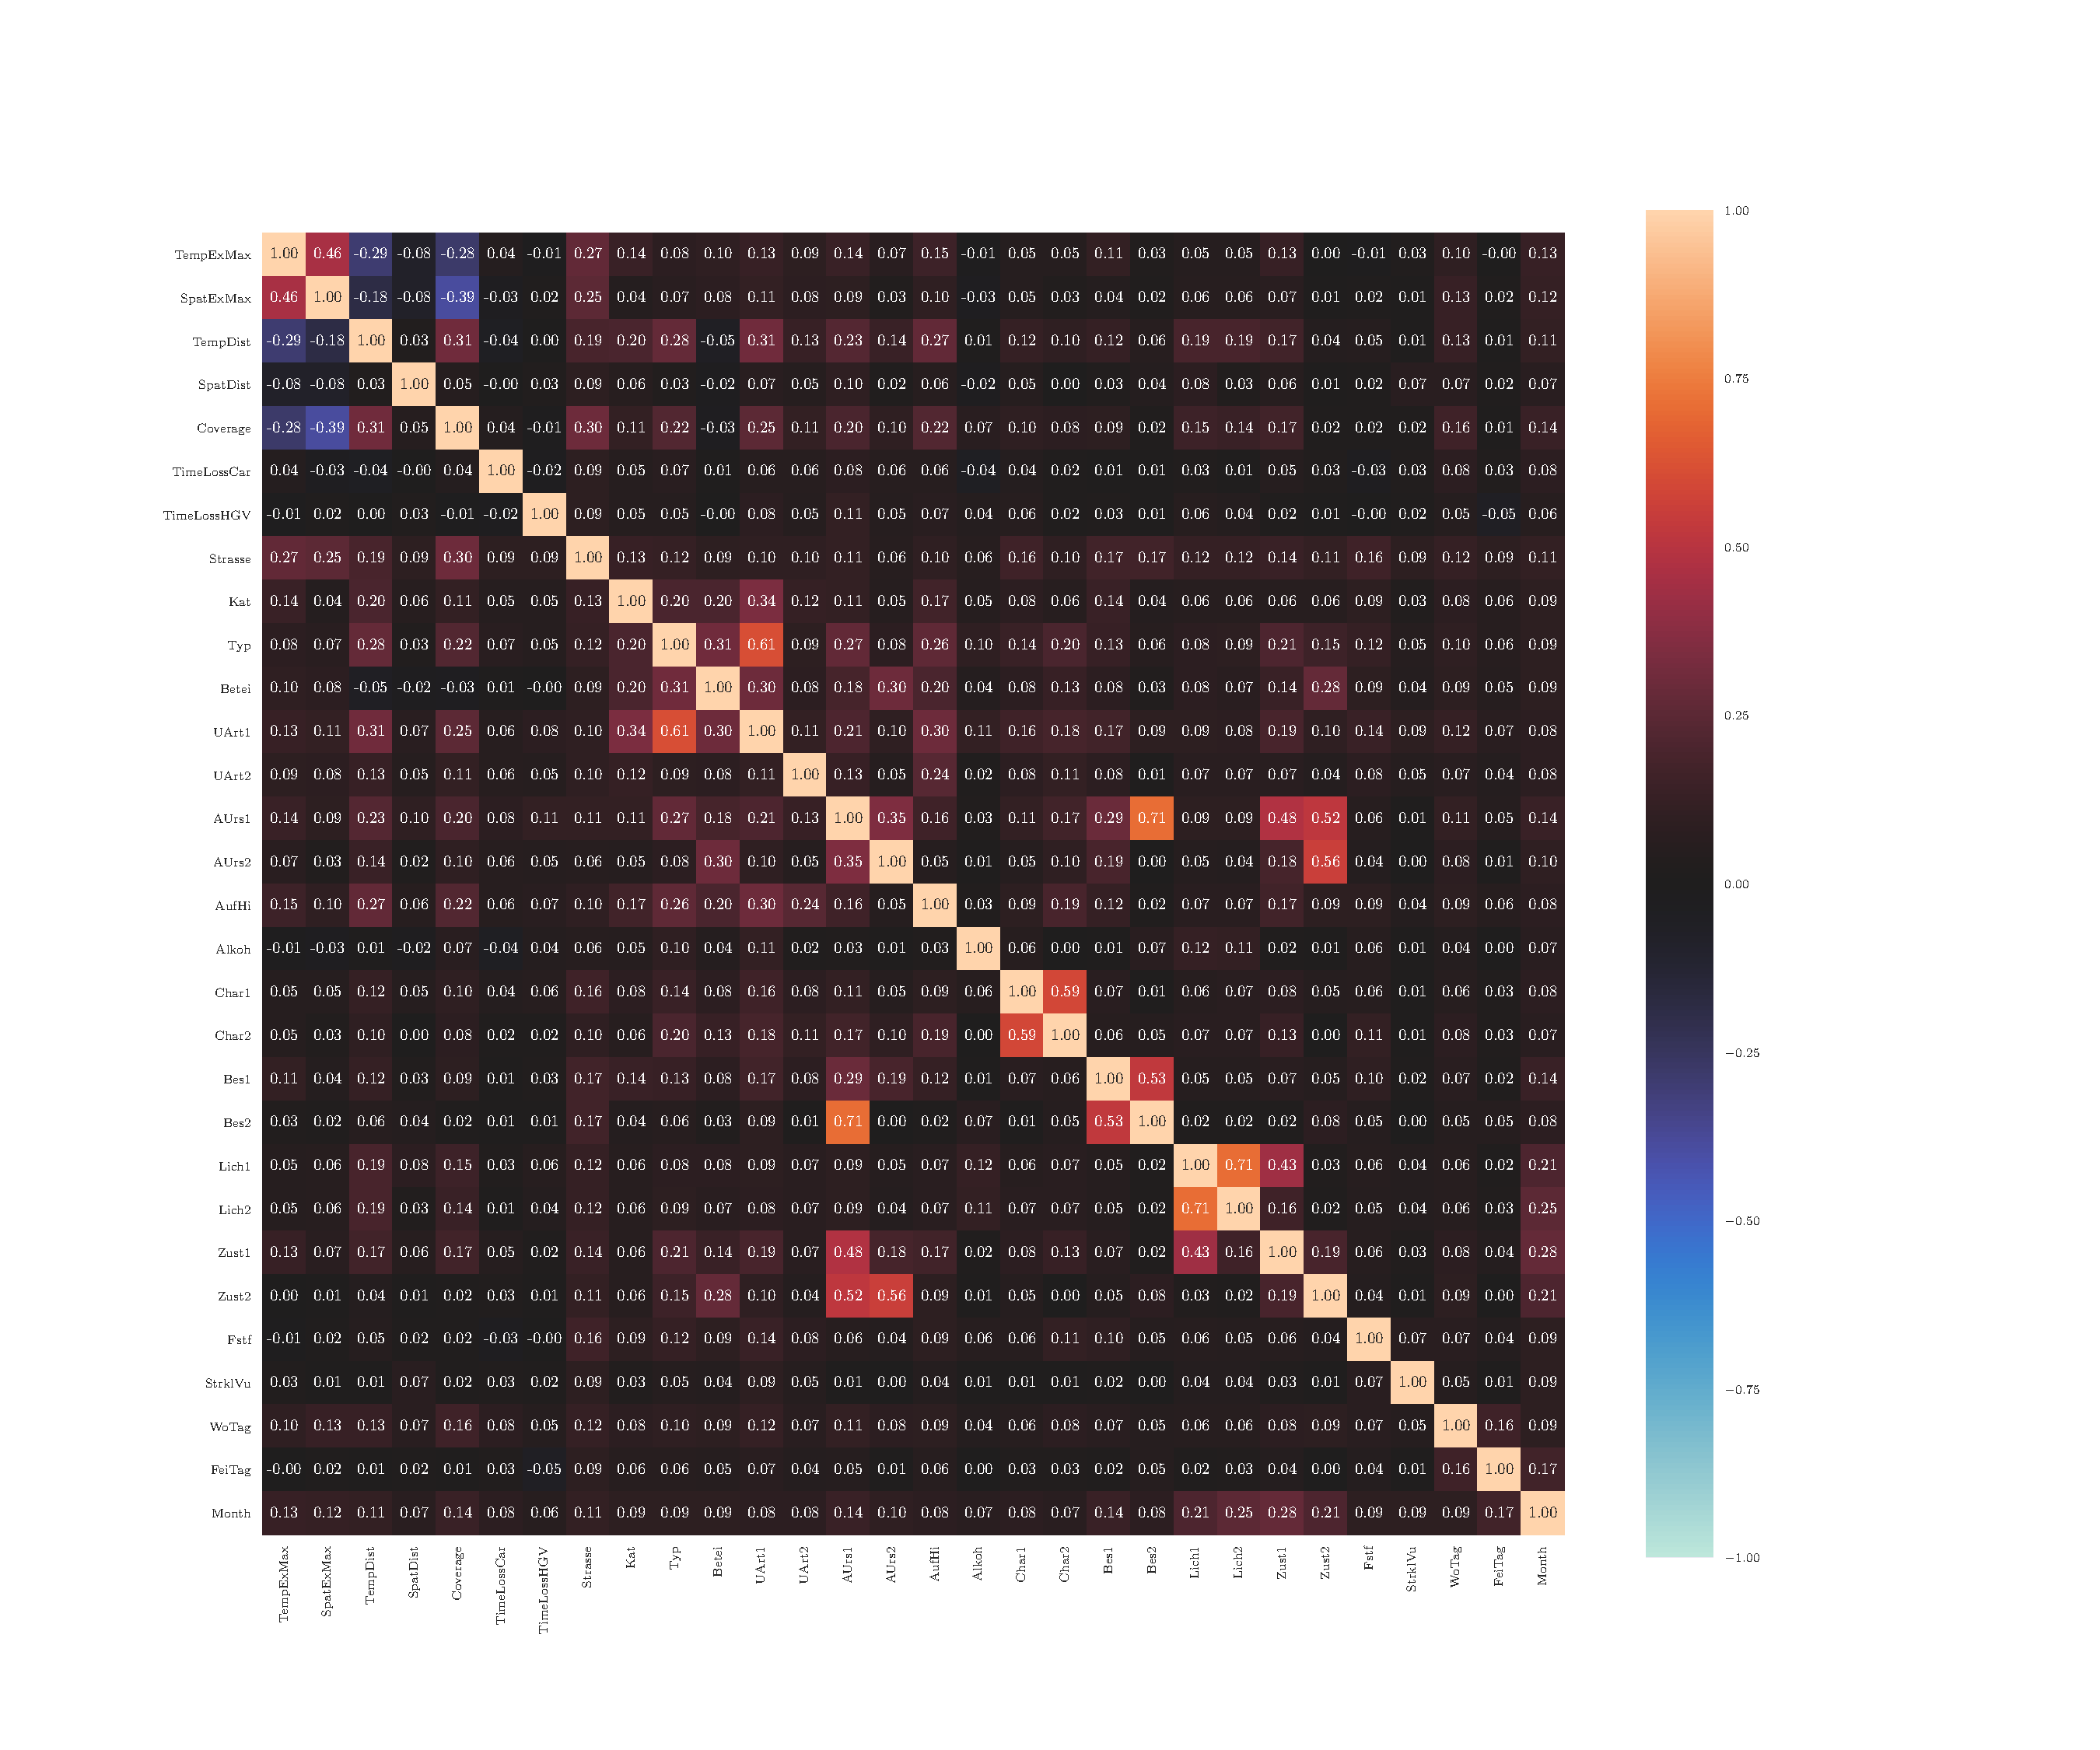
\includegraphics[scale=0.52, trim=3cm 2cm 0cm 0cm]{../CorrAnalysis/data/BAYSIS/02_matched/plots/baysis_matched_corr_cramers}
% 		\caption{Correlation matrix for BAYSIS matched data, with $V$, $\eta$, $\tau$, $r_{pq}$, $r$}
% 		\label{img:correlation_matrix_matched_cramers}
% 	\end{figure}
% \restoregeometry
\begin{figure}[!ht]
	\centering
	\makebox[\textwidth][c]{%
		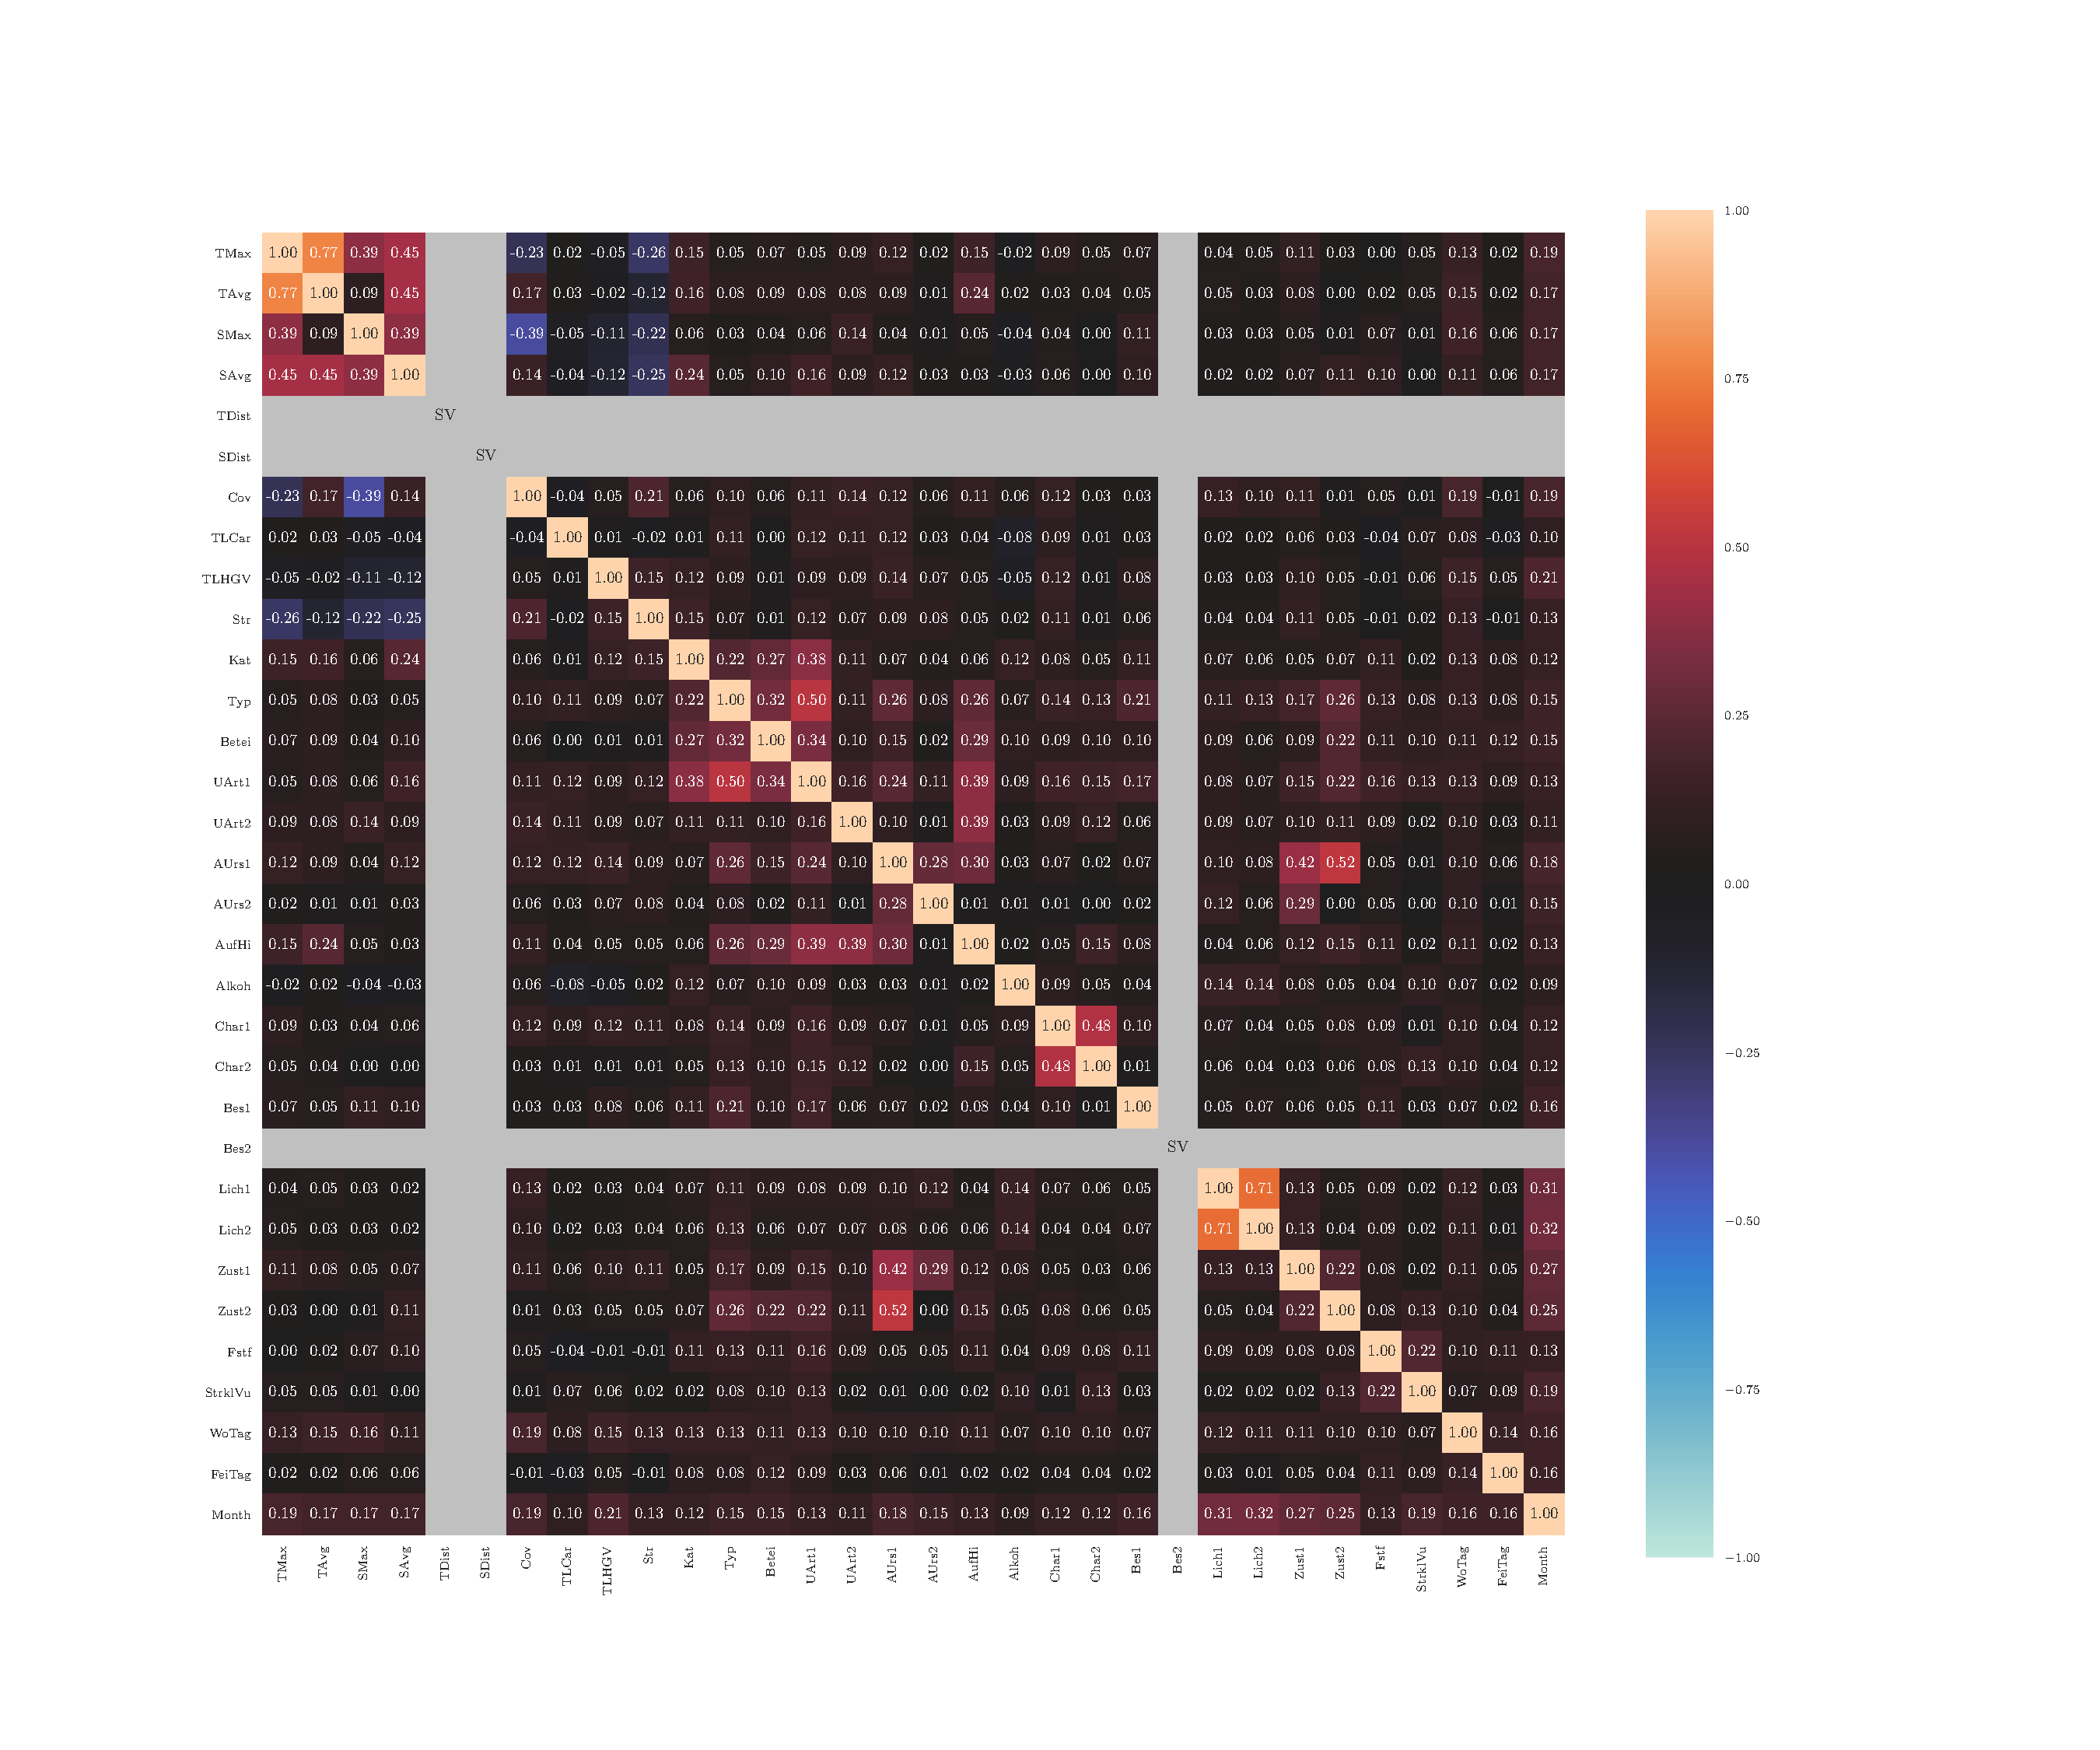
\includegraphics[width=1.4\textwidth, trim=0cm 2.5cm 6cm 3cm]{CorrAnalysis/data/BAYSIS/03_selected_02_duringJam/plots/baysis_selected_corr_cramers}%
	}
	\caption{Correlation matrix for congestion-accident matched data classified as \textit{Jam Effector}, with $V$, $\eta$, $\tau$, $r_{pq}$, $r$}
	\label{img:correlation_matrix_matched_cramers}
\end{figure}

\large
\centerline{\textbf{Strasse}}
\normalsize

\paragraph{Maximal temporal Extent:}
\paragraph{Average temporal Extent:}
\paragraph{Maximal spatial Extent:}
\paragraph{Average spatial Extent:}
\paragraph{Coverage}
\paragraph{Time-loss HGV}

\large
\centerline{\textbf{Kat}}
\normalsize

\paragraph{Maximal temporal Extent:}
\paragraph{Average temporal Extent:}
\paragraph{Average spatial Extent:}

\large
\centerline{\textbf{UArt1}}
\normalsize

\paragraph{Average spatial Extent:}

\large
\centerline{\textbf{UArt2}}
\normalsize

\paragraph{Maximal spatial Extent:}

\large
\centerline{\textbf{AufHi}}
\normalsize

\paragraph{Maximal temporal Extent:}
\paragraph{Average temporal Extent:}


\large
\centerline{\textbf{WoTag}}
\normalsize

\paragraph{Average temporal Extent:}
\paragraph{Maximal spatial Extent:}
\paragraph{Coverage}
\paragraph{Time-loss HGV}

\large
\centerline{\textbf{Month}}
\normalsize

\paragraph{Maximal temporal Extent:}
\paragraph{Average temporal Extent:}
\paragraph{Maximal spatial Extent:}
\paragraph{Average spatial Extent:}
\paragraph{Coverage}
\paragraph{Time-loss HGV}